\documentclass[conference,a4paper]{IEEEtran}
\IEEEoverridecommandlockouts
\usepackage[utf8]{inputenc}
\usepackage[T1]{fontenc}
\usepackage{amsmath,amssymb}
\usepackage{graphicx}
\usepackage{booktabs}
\usepackage{siunitx}
\usepackage{tikz}
\usetikzlibrary{arrows.meta,positioning,calc,fit}
\usepackage[hidelinks]{hyperref}
\usepackage{cite}
\graphicspath{{../figures/}}
\sisetup{detect-all, per-mode=symbol}

\begin{document}

\title{Smart HVAC Temperature Control and Fault Detection\\ on a Laboratory-Scale Thermal Chamber}

\author{
\IEEEauthorblockN{Somanshu Juneja (B24354)}
\IEEEauthorblockA{IIT Mandi}
\and
\IEEEauthorblockN{Ridhi Garg (B24348)}
\IEEEauthorblockA{IIT Mandi}
\and
\IEEEauthorblockN{Pramukto Mandal (B24347)}
\IEEEauthorblockA{IIT Mandi}
\thanks{EE302 Control Systems Laboratory, final project, Group~2, Problem Statement~4.}
}

\maketitle

\begin{abstract}
We design and evaluate temperature control and model-based fault detection for a laboratory-scale
HVAC chamber, the Quanser QNET HVAC Trainer driven by an NI ELVIS~II+ from MATLAB.
A first-order-plus-dead-time model identified from a \SI{3}{V} open-loop step test
($K=\SI{1.71}{\celsius\per\volt}$, $\tau=\SI{33.7}{s}$, 89\,\% fit) is implemented in Simulink and
used to tune a PI controller with the SIMC rules, which is compared with a hysteresis ON-OFF
controller in a \SI{2}{Hz} real-time loop. Airflow disturbances and faults are produced with
3D-printed plates over the fan. A nominal model running in parallel with the plant generates a
residual that is filtered, thresholded and classified. In eight hardware experiments, each replayed in
Simulink with identical inputs, the PI loop tracks setpoint steps without limit cycling and keeps the
chamber within \SI{0.35}{\celsius} of the setpoint while the fan is restricted or blocked, whereas
the ON-OFF loop oscillates by about \SI{0.8}{\celsius} and, because lamp power is nonlinear in the command, uses about twice the electrical energy. Restricted airflow, a blocked fan and a
\SI{2}{\celsius} sensor bias are all detected and correctly classified within
\SIrange{21.5}{38.5}{s}, with no alarm in the fault-free run. Making the detector reliable required
refitting its model on closed-loop data and referencing it to the chamber's resting temperature.
\end{abstract}

\begin{IEEEkeywords}
HVAC, PI control, SIMC tuning, system identification, fault detection, residual generation
\end{IEEEkeywords}

% =====================================================================
\section{Introduction}
Heating, ventilation and air-conditioning systems are among the largest energy consumers in
buildings, and many of their faults (clogged filters, failing fans, drifting sensors) go unnoticed
because the feedback loop quietly compensates for them~\cite{isermann2005}. A controller that hides a
fault while using more or less energy, or a sensor that reports a wrong temperature to a perfectly
working loop, cannot be seen from the setpoint error alone.

The objectives of this work are to (i) model the thermal behaviour of a small chamber and implement
the model in Simulink, (ii) compare ON-OFF control with a PI controller in simulation and on
hardware, (iii) assess the response to a controlled airflow disturbance, and (iv) detect and
classify safe fault conditions---restricted airflow, fan failure and sensor bias---while comparing
temperature performance and heater effort in normal and faulted operation.

% =====================================================================
\section{Hardware Design}\label{sec:setup}
\subsection{Chamber, sensors and actuators}
The chamber is the Quanser QNET HVAC Trainer: a Plexiglas duct with a halogen lamp acting as heater
at one end and a fixed-speed \SI{16}{V} fan at the other, a thermistor inside the duct and a second
thermistor outside it for ambient temperature~\cite{quanser}. The board plugs into an NI ELVIS~II+,
whose analog I/O is accessed from MATLAB through NI-DAQmx and the Data Acquisition Toolbox
(Fig.~\ref{fig:wiring}). The heater is driven through the board's PWM power amplifier from analog
output AO1. Each control step performs an on-demand read averaged over five scans; the loop period
is $T_s=\SI{0.5}{s}$. Table~\ref{tab:io} lists the channels and scalings used.

\begin{figure}[t]
\centering
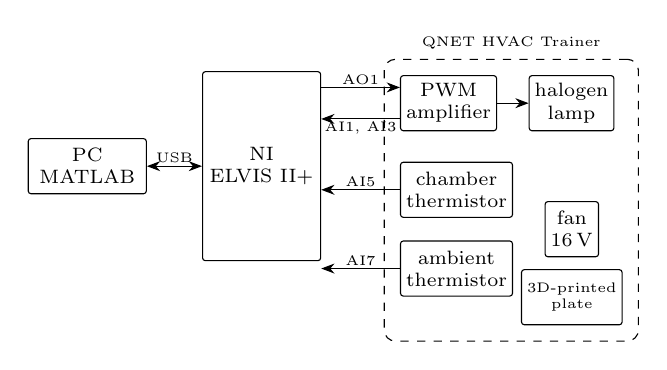
\begin{tikzpicture}[font=\scriptsize, >=Stealth,
  box/.style={draw, rounded corners=1pt, align=center, minimum height=7mm, inner sep=2pt},
  lab/.style={font=\tiny, inner sep=1pt}]
\node[box, minimum width=15mm] (pc) {PC\\MATLAB};
\node[box, right=7mm of pc, minimum width=15mm, minimum height=24mm] (elvis) {NI\\ELVIS II+};
\node[box, right=10mm of elvis, yshift=8mm] (amp) {PWM\\amplifier};
\node[box, right=4mm of amp] (lamp) {halogen\\lamp};
\node[box, right=10mm of elvis, yshift=-3mm] (tc) {chamber\\thermistor};
\node[box, right=10mm of elvis, yshift=-13mm] (ta) {ambient\\thermistor};
\node[box, right=4mm of ta, yshift=5mm] (fan) {fan\\\SI{16}{V}};
\node[box, below=1.5mm of fan, font=\tiny] (plate) {3D-printed\\plate};
\draw[<->] (pc) -- node[above, lab]{USB} (elvis);
\draw[->] ([yshift=2mm]elvis.east |- amp) -- node[above, lab]{AO1} ([yshift=2mm]amp.west);
\draw[<-] ([yshift=-2mm]elvis.east |- amp) -- node[below, lab]{AI1, AI3} ([yshift=-2mm]amp.west);
\draw[->] (amp) -- (lamp);
\draw[->] (tc) -- node[above, lab]{AI5} (elvis.east |- tc);
\draw[->] (ta) -- node[above, lab]{AI7} (elvis.east |- ta);
\node[draw, dashed, rounded corners, fit=(amp)(lamp)(tc)(ta)(fan)(plate), inner sep=2mm,
      label={[font=\tiny]above:QNET HVAC Trainer}] {};
\end{tikzpicture}
\caption{Wiring and signal flow of the real-time setup (AI1/AI3: heater current and voltage sense). The airflow plate slides over the fan face.}
\label{fig:wiring}
\end{figure}

\begin{table}[t]
\centering
\caption{I/O channels and scalings}\label{tab:io}
\begin{tabular}{@{}lll@{}}
\toprule
Signal & Channel & Scaling \\
\midrule
Heater command $u$ & AO1 & \SIrange{0}{5}{V} (capped) \\
Chamber temperature $T$ & AI5 & \SI{20}{\celsius\per\volt}, offset \SI{1.9}{\celsius} \\
Ambient temperature $T_a$ & AI7 & \SI{20}{\celsius\per\volt} \\
Heater current $I$ & AI1 & \SI{-0.22}{A\per V} (provisional) \\
Heater voltage $V_h$ & AI3 & \num{-3.33} (provisional) \\
\bottomrule
\end{tabular}
\end{table}

\subsection{Fabricated parts: airflow plates}
Because the fan speed cannot be set in software, airflow changes are made physically with slip-on
caps for the fan face, designed parametrically in OpenSCAD and 3D-printed. Each cap is a square
sleeve that slides \SI{8}{mm} over the fan housing with \SI{0.6}{mm} clearance per side and a
\SI{2}{mm} face plate with a central hole whose area is a chosen fraction of the blade opening
($d = d_{\mathrm{fan}}\sqrt{f}$), plus finger notches and an engraved label. Three versions were
produced: $f=1$ (frame only, fit check), $f=0.5$ (disturbance and restricted airflow) and $f=0$
(fan-failure emulation). They are printed face-down without supports and fitted only at the fan end,
at least \SI{5}{cm} from the lamp (Fig.~\ref{fig:plates}).

\begin{figure}[t]
\centering
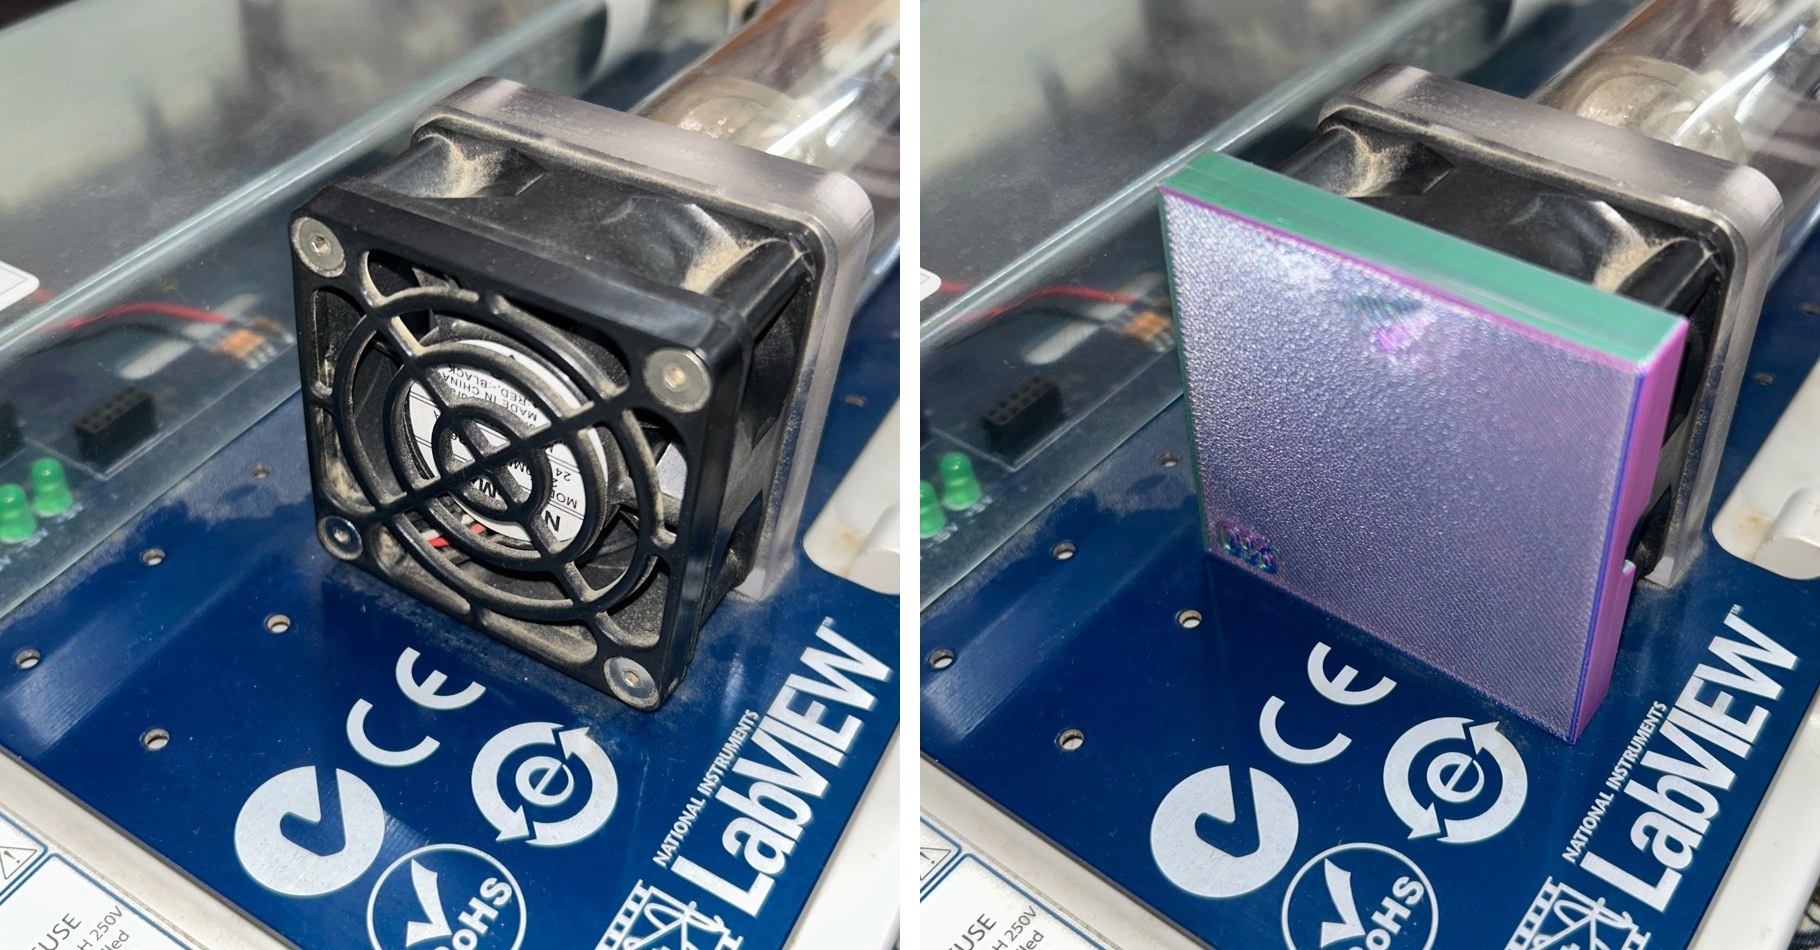
\includegraphics[width=\columnwidth]{fan_plate_photos}
\caption{Fan end of the QNET HVAC Trainer without a plate (left) and with the closed 0\,\% plate
fitted for fan-failure emulation (right).}\label{fig:plates}
\end{figure}

\subsection{Safety}
The heater command is capped at \SI{5}{V}. The heater is forced off when the raw chamber reading
exceeds \SI{45}{\celsius} or ambient plus \SI{20}{\celsius}, on any read error, on a stop key and when
any script exits. The sensor-bias fault is injected in software only into the signal seen by the
controller and detector; the safety logic always uses the raw reading.

% =====================================================================
\section{Thermal Model and Identification}\label{sec:model}
The chamber is treated as a single thermal node: heat enters from the lamp and is carried away by
the airflow,
\begin{equation}
\tau\,\dot T(t) = K\,u(t-L) - a(t)\,\bigl(T(t)-T_a\bigr),\label{eq:plant}
\end{equation}
where $\tau$ is the product of thermal capacitance and resistance, $K$ the steady-state gain, $L$ a
dead time and $a$ an airflow factor ($a=1$ normal, $a<1$ restricted). In steady state
$T-T_a=Ku/a$, so restricted airflow raises the temperature reached for a given heater command.

The parameters were identified from an open-loop test: \SI{60}{s} at rest, a \SI{3}{V} step for
\SI{300}{s}, then \SI{240}{s} of cooling, sampled at \SI{0.5}{s}. Minimising the squared output
error with Nelder--Mead gives $K=\SI{1.709}{\celsius\per\volt}$, $\tau=\SI{33.7}{s}$ and
$L=\SI{0.19}{s}$ (rounded up to one sample) with a normalised fit of 89.0\,\% (Fig.~\ref{fig:ident}).
The temperature fluctuations between \SIlist{200;350}{s}, caused by turbulent airflow in the duct,
are not captured by the linear model.

\begin{figure}[t]
\centering
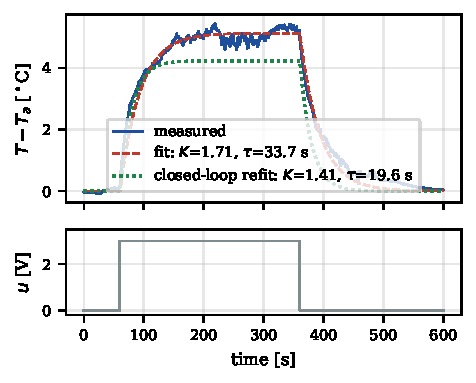
\includegraphics[width=\columnwidth]{identification}
\caption{Open-loop \SI{3}{V} step test with the identified model, and the model refitted on
closed-loop data that the fault detector uses.}\label{fig:ident}
\end{figure}

The closed-loop runs later showed the plant to be weaker and faster than the step test suggested. A
second fit of $K$ and $\tau$ on the two tracking runs gives $K=\SI{1.41}{\celsius\per\volt}$ and
$\tau=\SI{19.6}{s}$. This model is used by the fault detector, while the controller keeps the gains
derived from the step test (Section~\ref{sec:lessons}).

\subsection{Simulink implementation}
The model is built by a script from standard Simulink blocks (Fig.~\ref{fig:simulink}): a transport
delay, the heat balance~\eqref{eq:plant} with time-varying $a(t)$ and an integrator, a \SI{1}{s}
sensor lag, an additive sensor-bias input, both controllers selected by a switch, actuator
saturation, and the nominal model and residual filter of the fault detector. The same parameter file
feeds the simulation and the hardware loop. For every hardware run, the analysis script replays the
experiment with the same reference, controller and logged times of plate insertion and bias, so the
two are directly comparable.

\begin{figure*}[t]
\centering
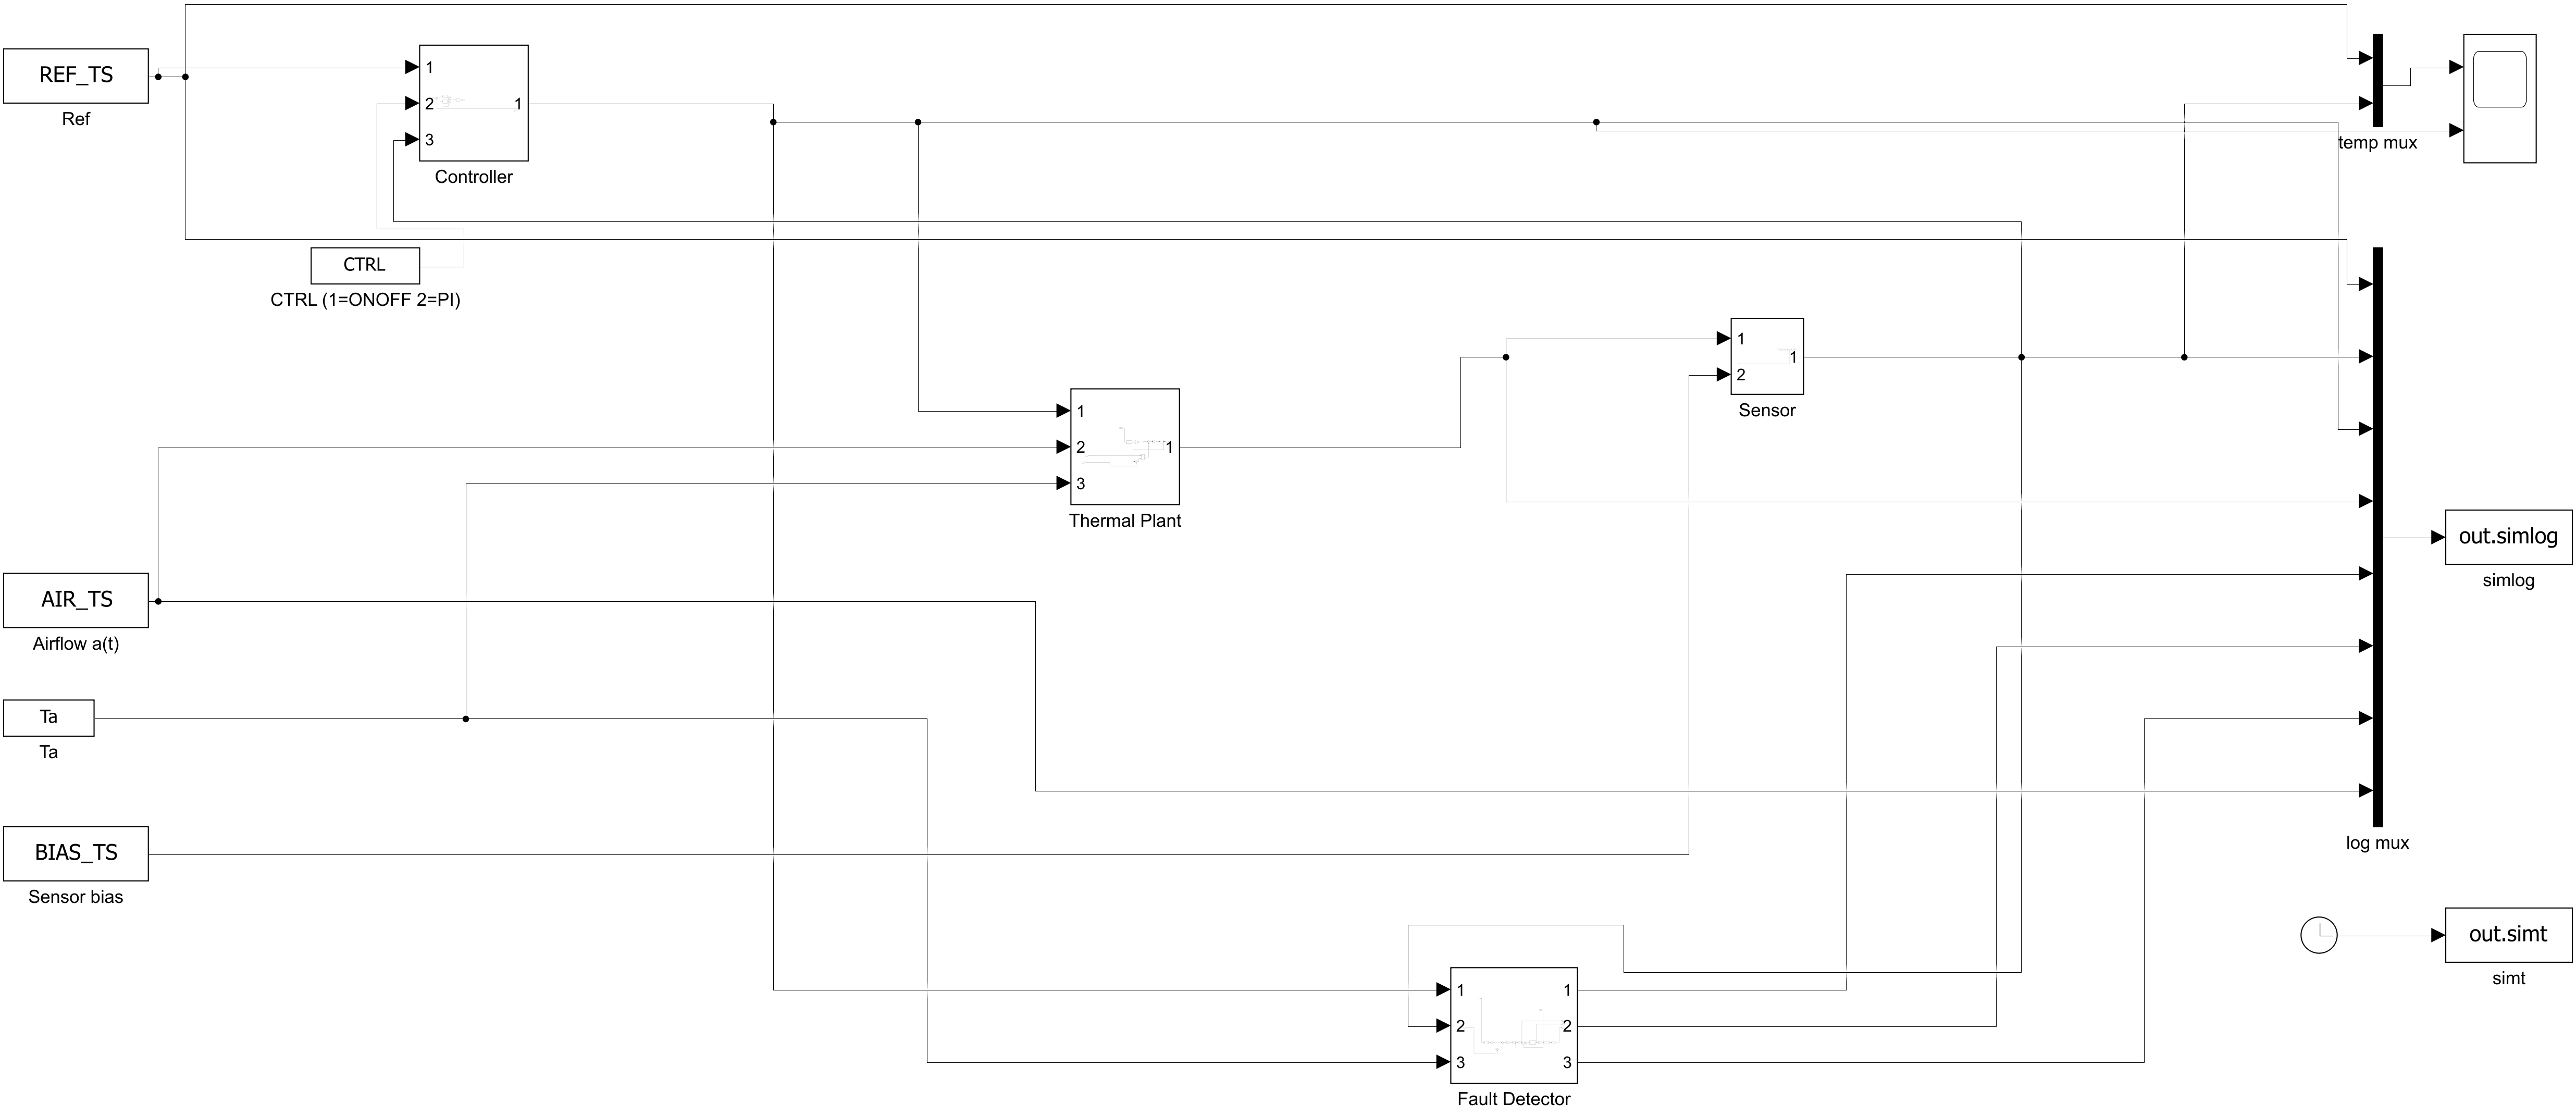
\includegraphics[width=0.66\textwidth]{simulink}\hfill
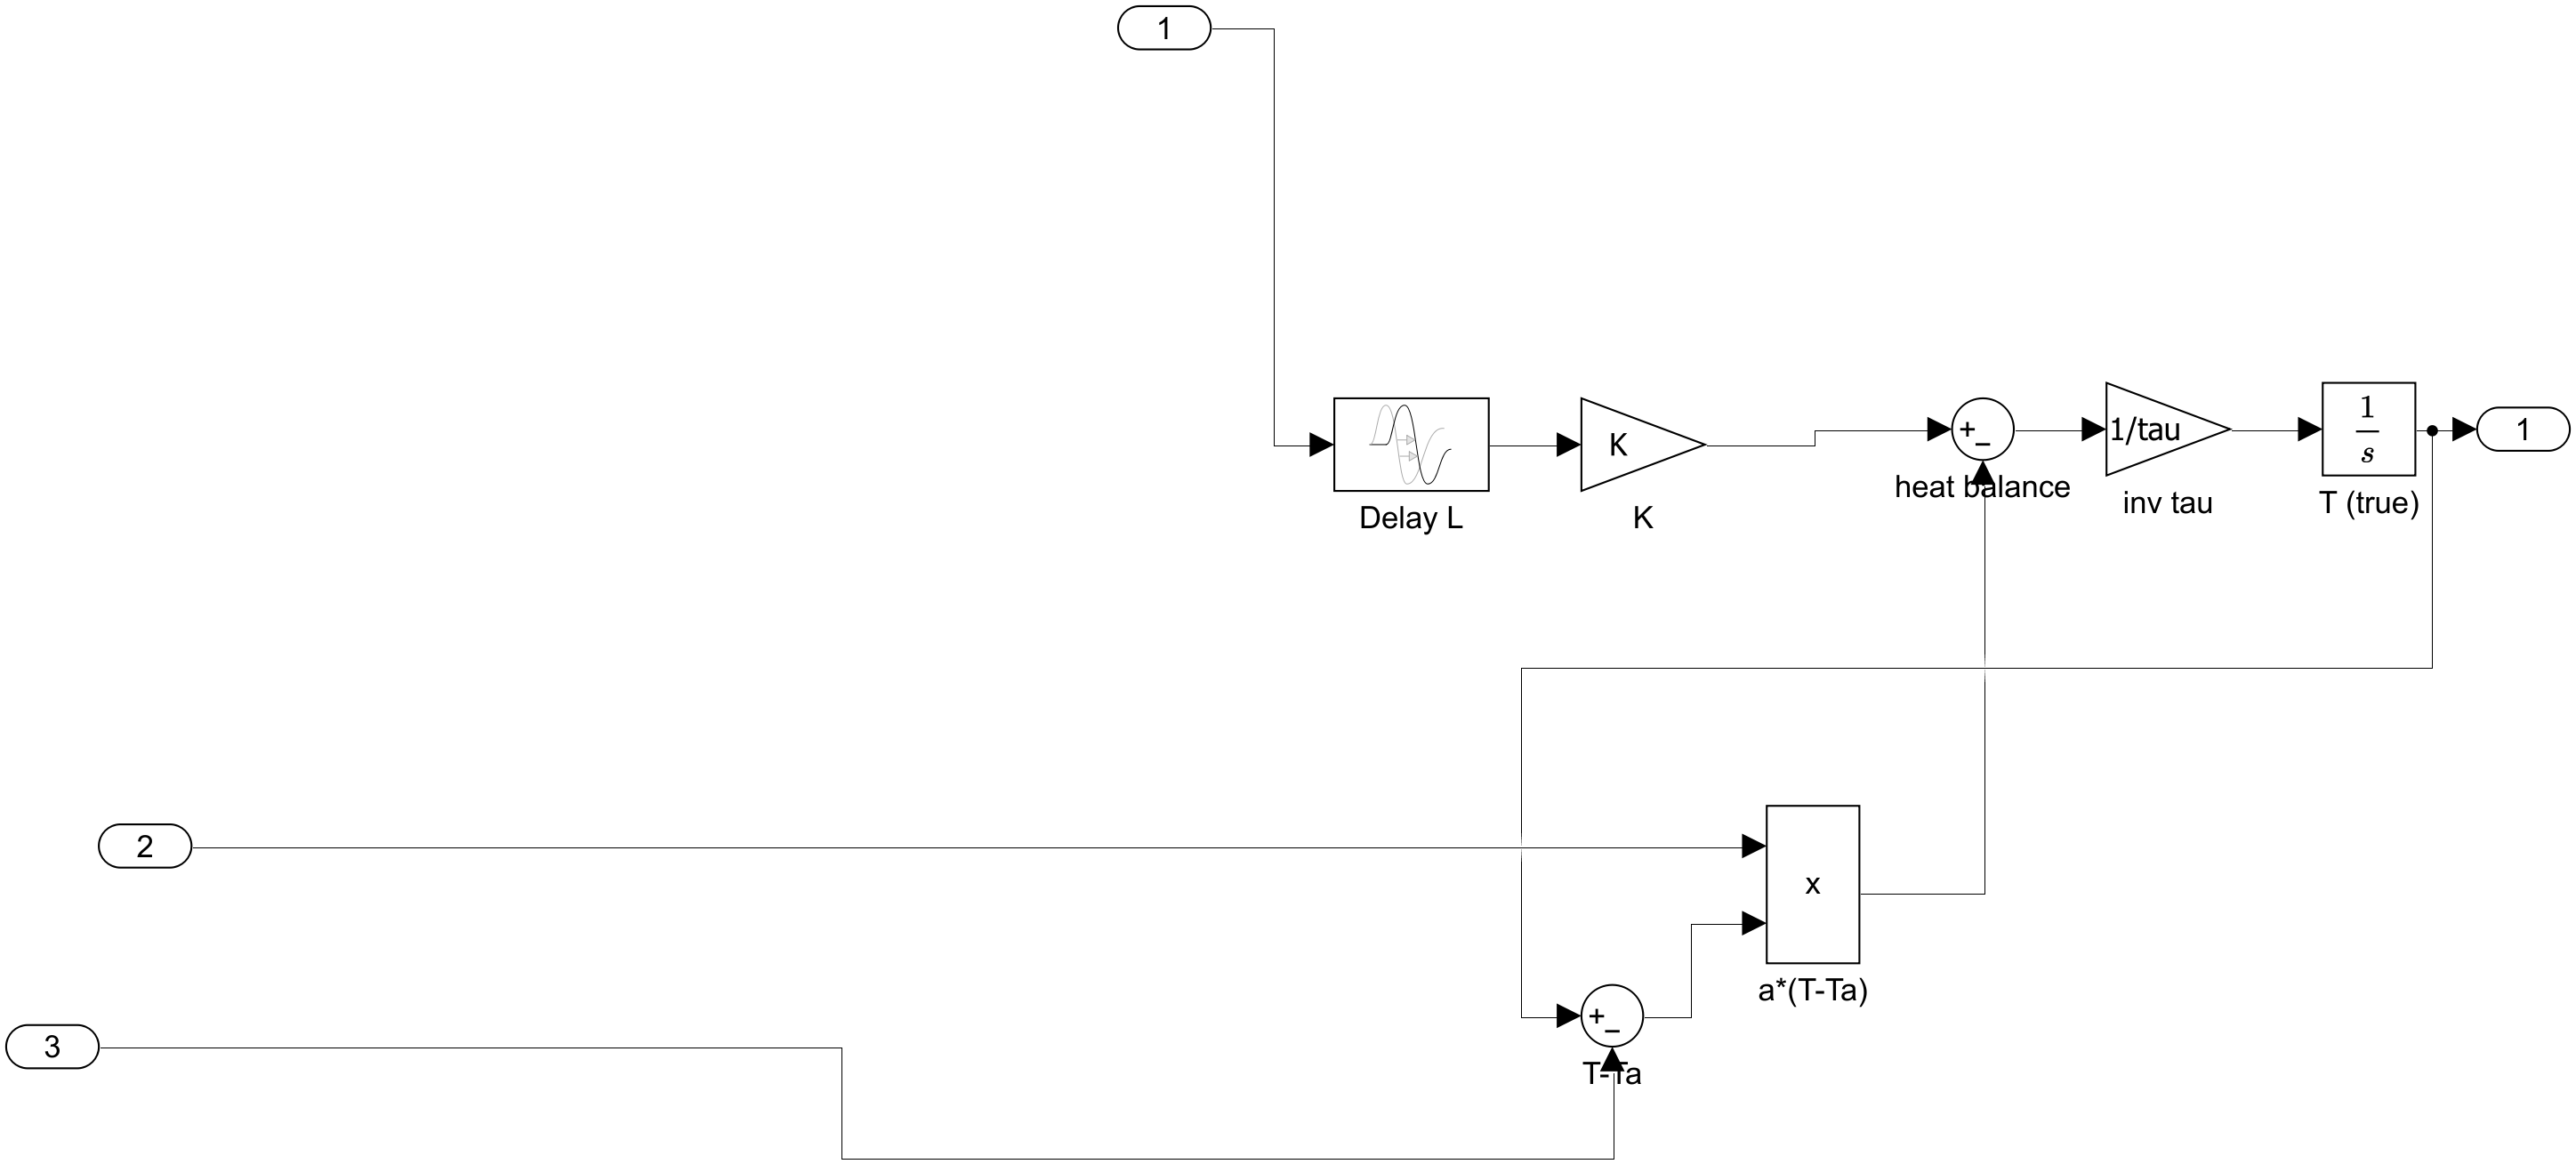
\includegraphics[width=0.32\textwidth]{simulink_plant}
\caption{Simulink model. Left: controller, thermal plant, sensor (lag and bias) and fault detector
subsystems with the scenario inputs. Right: the thermal-plant subsystem implementing~\eqref{eq:plant}.}
\label{fig:simulink}
\end{figure*}

% =====================================================================
\section{Controller Design}\label{sec:control}
\subsection{ON-OFF with hysteresis}
The heater is switched fully on (\SI{5}{V}) when the error $e=r-T$ exceeds $+H/2$ and off when it
falls below $-H/2$, with $H=\SI{0.6}{\celsius}$. The hysteresis limits the switching rate at the
cost of a sustained limit cycle.

\subsection{PI with SIMC tuning}
The PI law $u = K_p e + K_i\!\int e\,dt$ is tuned with Skogestad's SIMC rules~\cite{skogestad2003}
for a first-order-plus-dead-time plant with closed-loop time constant $\tau_c=\max(\tau/4,\,2L)$:
\begin{equation}
K_p = \frac{\tau}{K(\tau_c+L)},\qquad T_i=\min\bigl(\tau,\,4(\tau_c+L)\bigr).
\end{equation}
With the step-test model, $K_p=\SI{2.21}{V\per\celsius}$, $T_i=\SI{33.7}{s}$ and
$K_i=\SI{0.0655}{V\per(\celsius\,s)}$. The integral is updated with forward Euler at $T_s$; the
output is limited to \SIrange{0}{5}{V}, and integration is frozen while the output is saturated in
the direction of the error (clamping anti-windup)~\cite{astrom2006}.

% =====================================================================
\section{Fault Detection}\label{sec:fd}
\begin{figure}[t]
\centering
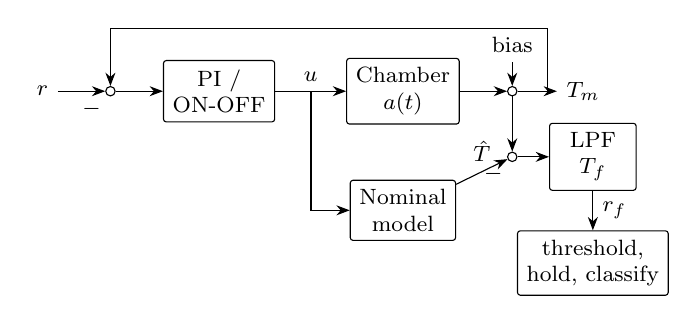
\begin{tikzpicture}[font=\footnotesize, >=Stealth, node distance=5mm and 6mm,
  blk/.style={draw, rounded corners=1pt, minimum height=6mm, minimum width=11mm, align=center},
  sum/.style={draw, circle, inner sep=1.2pt}]
\node (ref) {$r$};
\node[sum, right=of ref] (s1) {};
\node[blk, right=of s1] (ctl) {PI /\\ON-OFF};
\node[blk, right=9mm of ctl] (plant) {Chamber\\$a(t)$};
\node[sum, right=of plant] (s2) {};
\node[right=5mm of s2] (y) {$T_m$};
\node[blk, below=7mm of plant] (mdl) {Nominal\\model};
\node[sum, below=7mm of s2] (s3) {};
\node[blk, right=4mm of s3] (lpf) {LPF\\$T_f$};
\node[blk, below=5mm of lpf, minimum width=16mm] (dec) {threshold,\\hold, classify};
\node[above=3mm of s2] (bias) {bias};
\draw[->] (ref) -- (s1);
\draw[->] (s1) -- (ctl);
\draw[->] (ctl) -- node[above]{$u$} (plant);
\draw[->] (plant) -- (s2);
\draw[->] (bias) -- (s2);
\draw[->] (s2) -- (y);
\draw[->] ($(s2)!0.5!(y)$) |- ++(0,8mm) -| (s1) node[below left]{$-$};
\draw[->] ($(ctl)!0.5!(plant)$) |- (mdl);
\draw[->] (mdl) -- node[above]{$\hat T$} (s3) node[below left]{$-$};
\draw[->] (s2) -- (s3);
\draw[->] (s3) -- (lpf);
\draw[->] (lpf) -- node[right]{$r_f$} (dec);
\end{tikzpicture}
\caption{Control loop and residual generator. The nominal model receives the same heater command as
the plant and assumes normal airflow and no sensor bias.}\label{fig:block}
\end{figure}

A nominal copy of~\eqref{eq:plant} with $a=1$ runs in parallel with the plant, driven by the same
heater command (Fig.~\ref{fig:block}). The residual $r=T_m-\hat T$ is low-pass filtered,
\begin{equation}
r_f[k] = r_f[k-1] + \alpha\,(r[k]-r_f[k-1]),\qquad \alpha = 1-e^{-T_s/T_f},
\end{equation}
with $T_f=\SI{20}{s}$. An alarm is raised when $|r_f|>R_{th}=\SI{1.3}{\celsius}$ for at least
$T_{hold}=\SI{15}{s}$, after an arming delay of \SI{60}{s}. Faults are classified as follows:
\begin{itemize}
\item a jump of more than \SI{1}{\celsius} between two samples within the preceding \SI{90}{s}:
\emph{sensor bias / sensor fault};
\item otherwise $r_f>0$ (chamber hotter than the model): \emph{low airflow};
\item otherwise $r_f<0$: \emph{excess cooling / weak heater};
\item independently, $u>\SI{0.5}{V}$ with heater current below \SI{0.05}{A} for \SI{15}{s}:
\emph{heater fault}.
\end{itemize}
The same function runs in the simulation and on the hardware.

A restricted fan lowers $a$, so for the same heater command the chamber settles hotter than the
nominal model and $r_f$ becomes positive. In closed loop, the controller brings $T$ back to the
setpoint by reducing $u$, which drives the nominal model \emph{down}; the residual therefore persists,
and the fault stays visible even though the controller has removed it from the setpoint error.

% =====================================================================
\section{Results}\label{sec:results}
Each hardware run lasts \SI{1200}{s} and starts from a chamber that has stopped cooling. Tracking
runs use a staircase of \SIlist{+4;+6;+3}{\celsius} above ambient at \SIlist{20;420;820}{s};
disturbance and fault runs hold \SI{+5}{\celsius} and apply the plate or bias at about \SI{400}{s}.
Every run logs reference, measured and raw temperature, ambient, heater command, heater current and
voltage, model prediction, residual, fault flag and every key event.

\subsection{Setpoint tracking}
\begin{figure*}[t]
\centering
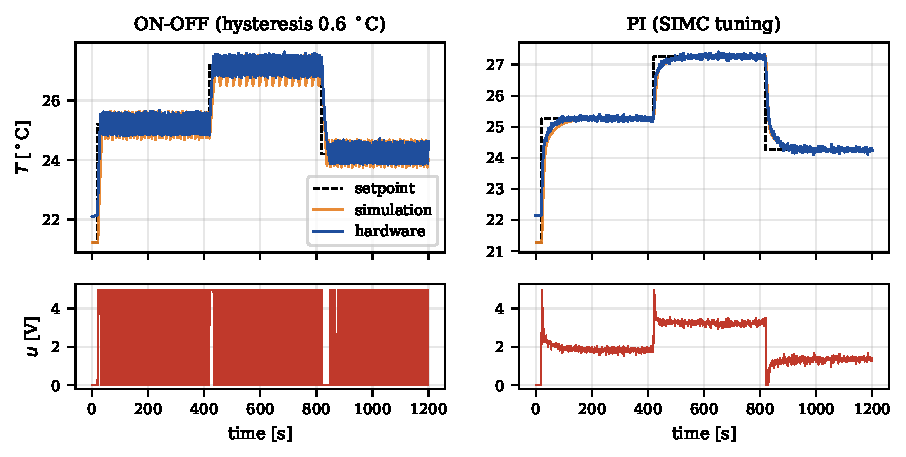
\includegraphics[width=\textwidth]{tracking}
\caption{Setpoint tracking on hardware and in simulation. Left: ON-OFF; right: PI.}\label{fig:track}
\end{figure*}

\begin{table*}[t]
\centering
\caption{Tracking metrics on hardware (simulation in brackets); settling band \SI{\pm0.5}{\celsius},
ripple = peak-to-peak over the last 20\,\% of each step}\label{tab:track}
\begin{tabular}{@{}llccccc@{}}
\toprule
 & Step [$^\circ$C] & Rise [s] & Settle [s] & OS [\%] & $e_{ss}$ [$^\circ$C] & Ripple [$^\circ$C] \\
\midrule
ON-OFF & 0.0$\to$4.0 & 8.0 (13.0) & 7.5 (362.5) & 12.2 (11.4) & 0.00 (0.04) & 0.80 (0.97) \\
 & 4.0$\to$6.0 & 9.0 (16.0) & 7.5 (393.0) & 22.5 (16.3) & 0.00 (0.17) & 0.82 (1.01) \\
 & 6.0$\to$3.0 & 18.0 (10.5) & 207.0 (12.5) & 11.7 (15.0) & 0.01 (-0.02) & 0.78 (0.93) \\
\midrule
PI & 0.0$\to$4.0 & 24.0 (40.5) & 22.5 (34.5) & 3.3 (0.0) & 0.00 (0.00) & 0.22 (0.00) \\
 & 4.0$\to$6.0 & 27.0 (42.5) & 13.5 (16.5) & 7.7 (0.0) & 0.01 (0.00) & 0.23 (0.00) \\
 & 6.0$\to$3.0 & 36.5 (36.5) & 29.0 (20.5) & 5.7 (0.0) & 0.00 (0.00) & 0.27 (0.00) \\
\bottomrule
\end{tabular}

\end{table*}

Fig.~\ref{fig:track} and Table~\ref{tab:track} compare the two controllers. The ON-OFF loop
reaches each new setpoint fastest (rise times of \SIrange{8}{18}{s}) because it always applies full
power, but it overshoots by \SIrange{12}{23}{\percent} of the step and then oscillates with a
peak-to-peak ripple of about \SI{0.8}{\celsius}. Its settling time is therefore sensitive to how the
ripple sits relative to the \SI{\pm0.5}{\celsius} band: \SI{7.5}{s} on the up-steps on hardware, but
\SI{207}{s} on the down-step and over \SI{360}{s} in simulation, where the simulated ripple is slightly
larger. The PI loop rises in \SIrange{24}{37}{s}, overshoots by \SIrange{3}{8}{\percent}, settles in
\SIrange{13.5}{29}{s} and has no limit cycle; the remaining \SI{0.2}{\celsius} peak-to-peak variation
is sensor noise and airflow turbulence. Both controllers have negligible steady-state error.

Simulation and hardware agree in shape; the hardware PI response rises faster than simulated
(\SI{24}{s} versus \SI{40.5}{s} on the first step) because the real chamber is faster than the
step-test model ($\tau=\SI{19.6}{s}$ versus \SI{33.7}{s}, Section~\ref{sec:model}), and the
simulated PI response is smoother because the model has no measurement noise.

Over the tracking run both controllers used almost the same mean command (\SI{2.23}{V} for ON-OFF,
\SI{2.25}{V} for PI), yet the measured electrical energy was \SI{1760}{J} for ON-OFF and \SI{861}{J}
for PI. Lamp power grows roughly with the square of the applied voltage, so switching between
\SI{0}{V} and \SI{5}{V} delivers more power than a steady command with the same mean. Given the
provisional scaling of the power sensing, the ratio is more reliable than the absolute values.

\subsection{Disturbance rejection}
\begin{figure*}[t]
\centering
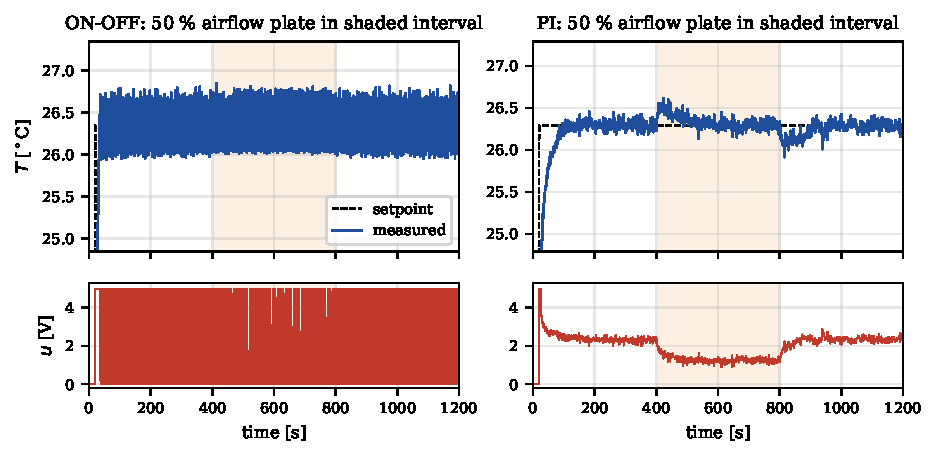
\includegraphics[width=\textwidth]{disturbance}
\caption{Response to the 50\,\% airflow plate (shaded), inserted at about \SI{400}{s} and removed
at about \SI{800}{s}.}\label{fig:dist}
\end{figure*}
Inserting the 50\,\% plate reduces the heat removed, so both controllers must cut the heater power
(Fig.~\ref{fig:dist}). The PI controller lowers its mean command from \SI{2.4}{V} to \SI{1.3}{V};
the temperature rises by at most \SI{0.32}{\celsius} and never leaves the \SI{\pm0.5}{\celsius}
band. The ON-OFF controller halves its duty cycle (47\,\% to 23\,\%) and keeps the mean on the
setpoint, but its ripple remains, with a peak deviation of \SI{0.50}{\celsius} after insertion. In
both runs the detector reports \emph{low airflow} \SIrange{30}{32}{s} after insertion and clears
after the plate is removed. In simulation, the same experiment with the estimated airflow factor
reproduces the drop in heater command and the residual step.

\subsection{Fault detection}
\begin{figure*}[t]
\centering
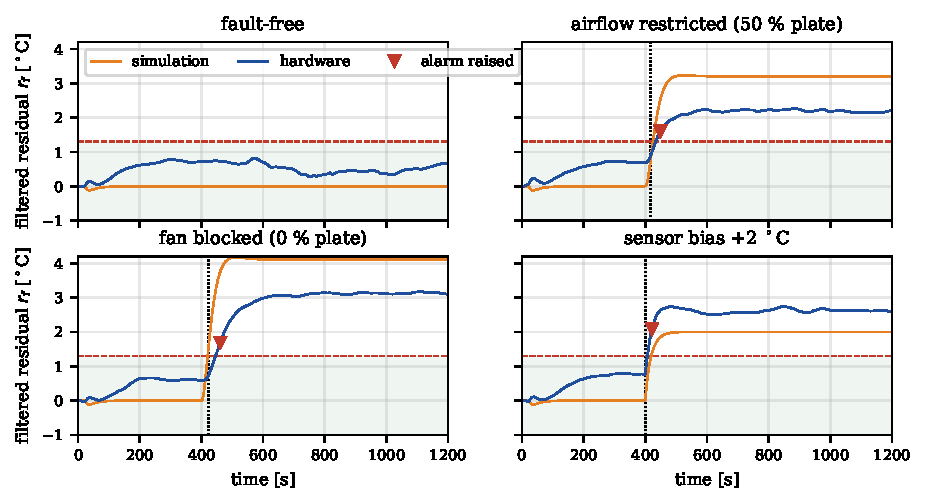
\includegraphics[width=\textwidth]{faults}
\caption{Filtered residual for the fault-free run and the three emulated faults under PI control
(dotted: fault applied; triangle: alarm; dashed: threshold $\pm R_{th}$).}\label{fig:faults}
\end{figure*}

\begin{table}[t]
\centering
\caption{Fault detection on hardware (simulated delay in brackets)}\label{tab:faults}
\setlength{\tabcolsep}{3pt}
\begin{tabular}{@{}lccl@{}}
\toprule
Run & Fault at & Delay & Classification \\
\midrule
Fault-free (PI)        & --              & no alarm              & -- \\
Restricted, 50\,\% (PI)& \SI{416.5}{s}   & \SI{32.0}{s} (39.5)   & low airflow \\
Blocked, 0\,\% (PI)    & \SI{422.5}{s}   & \SI{38.5}{s} (35.0)   & low airflow \\
Sensor bias (PI)       & \SI{400.0}{s}   & \SI{21.5}{s} (34.0)   & sensor bias \\
Disturbance (ON-OFF)   & \SI{404.5}{s}   & \SI{32.0}{s}          & low airflow \\
Disturbance (PI)       & \SI{406.5}{s}   & \SI{30.0}{s}          & low airflow \\
\bottomrule
\end{tabular}
\end{table}

All faults are detected and correctly classified (Table~\ref{tab:faults}, Fig.~\ref{fig:faults}).
In the fault-free run the filtered residual stays below \SI{0.82}{\celsius}, a margin of about
\SI{0.5}{\celsius} to the threshold. The two airflow faults produce residuals of about
\SI{+2.2}{\celsius} and \SI{+3.1}{\celsius}. From the steady-state heater commands, the airflow
factor is estimated as $a\approx0.36$ for the 50\,\% plate and $a\approx0.18$ for the closed plate;
these values replaced the initial guesses (0.6 and 0.25) in the simulation. The sensor bias is
detected fastest because it produces an immediate \SI{2}{\celsius} step in the residual, and the
jump test labels it correctly. Since the detector remembers the jump for only \SI{90}{s}, the label
later changes to \emph{low airflow}: the fault stays flagged, but its classification is reliable only
at onset. For the blocked fan, the plate event was logged three times (on at \SI{422.5}{s}, off at
\SI{425.5}{s}, on at \SI{433.5}{s}) while the plate was being fitted; the delay is quoted from the
first event and is \SI{27.5}{s} measured from the last.

\subsection{Normal versus faulted operation: energy and performance}
\begin{table}[t]
\centering
\caption{Heater use and tracking error after the fault ($t\geq\SI{450}{s}$), measured and true (raw sensor), hardware}\label{tab:energy}
\setlength{\tabcolsep}{3pt}
\begin{tabular}{@{}lcccc@{}}
\toprule
PI run & $\bar u$ [V] & Duty [\%] & $|e|$ meas./true [$^\circ$C] & $E^\dagger$ [J] \\
\midrule
fault-free & 2.53 & 51 & 0.04 / 0.04 & 1059 \\
restricted 50\,\% & 1.29 & 26 & 0.04 / 0.04 & 473 \\
fan blocked & 0.68 & 14 & 0.07 / 0.07 & 398 \\
sensor bias & 1.19 & 24 & 0.03 / 2.00 & 492 \\
\bottomrule
\multicolumn{5}{@{}l}{\footnotesize $^\dagger$whole run; provisional current/voltage scaling}
\end{tabular}

\end{table}

Table~\ref{tab:energy} compares heater use across runs. At a constant setpoint, the airflow faults
roughly halve (restricted) or quarter (blocked) the heater command needed, so a sustained drop in
heater effort is itself a symptom of reduced airflow, and running with a blocked fan would mask the
fault while appearing to save energy. The sensor-bias run shows the opposite hazard: the measured
temperature stays on the setpoint, but the controller is regulating a reading that is
\SI{2}{\celsius} too high, so the true chamber temperature settles \SI{2}{\celsius} \emph{below} the
setpoint (\SI{24.3}{\celsius} instead of \SI{26.3}{\celsius}) with correspondingly lower heater
effort. Neither problem is visible in the tracking error; both are visible in the residual. The
electrical energy uses the current and voltage sense channels, whose scalings are provisional, so
absolute joule values are approximate, whereas the command-based effort and duty cycle are exact.

% =====================================================================
\section{Making the Detector Work on Hardware}\label{sec:lessons}
\begin{figure}[t]
\centering
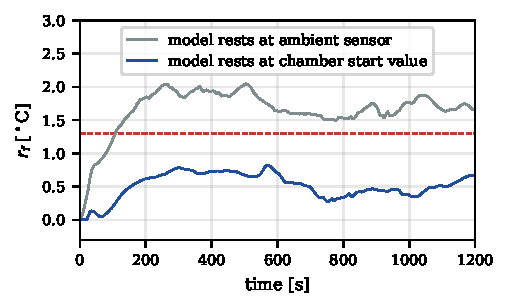
\includegraphics[width=\columnwidth]{rest_fix}
\caption{Fault-free PI run: residual with the nominal model resting at the ambient-sensor reading
(grey, earlier run) and at the chamber's own starting value (blue).}\label{fig:restfix}
\end{figure}
Two changes were needed before the detector stopped raising false alarms.

\emph{Model gain.} With the step-test model, the residual of the first tracking runs drifted to
\SI{-2.4}{\celsius} without any fault, and the detector reported \emph{excess cooling}. In closed loop
the ratio $(T-T_a)/u$ was about \SI{1.3}{\celsius\per\volt} instead of 1.71. Refitting $K$ and $\tau$
on the closed-loop data kept the fault-free residual within about \SI{\pm1}{\celsius}, and the
threshold was set to \SI{1.3}{\celsius}.

\emph{Resting reference.} With the heater off and the fan running, the chamber reading settled
between \SI{-0.2}{\celsius} and \SI{+1.0}{\celsius} relative to the ambient sensor on different
sessions. A nominal model that relaxes to the ambient reading turns this offset into a residual: in
one fault-free run it reached \SI{2.05}{\celsius} and was reported as \emph{low airflow}. Letting the
model relax to the chamber's own reading at the start of each run, after the chamber has stopped
cooling, removed the offset and reduced the peak residual of the same experiment to
\SI{0.82}{\celsius} (Fig.~\ref{fig:restfix}). A cooled-down chamber is therefore a precondition for
every run; the unattended runner enforces it by waiting until the temperature stops falling.

% =====================================================================
\section{Limitations}
\begin{itemize}
\item The single-node model cannot represent the temperature distribution along the duct, and the
lamp power is not linear in the command ($P\propto V^2$), which is one reason the gain identified at
\SI{3}{V} differs from the closed-loop gain.
\item The fan speed is fixed, so airflow can only be changed in discrete steps with the plates.
\item The sensor bias is injected in software rather than produced by a physical sensor fault.
\item Ambient temperature drifts during long runs, and the chamber's resting offset varies between
sessions; the detector's reference must be taken from a cooled chamber.
\item The heater current and voltage scalings are provisional, so the energy values are approximate.
\item The fault classification after the first \SI{90}{s} of a sensor fault falls back to the sign
test, and a heater fault was implemented but not staged.
\end{itemize}

% =====================================================================
\section{Conclusion}
A PI controller tuned with SIMC from a single step test gives smooth setpoint tracking and rejects
airflow disturbances to within \SI{0.35}{\celsius} on the QNET HVAC Trainer, clearly outperforming
a hysteresis ON-OFF controller in accuracy and, because the lamp power is nonlinear in the command,
using about half the measured electrical energy for the same tracking task. A residual-based detector built on the same kind of model
detects and classifies restricted airflow, a blocked fan and a sensor bias within about half a
minute without false alarms, provided its model is calibrated on closed-loop data and referenced to
the chamber's resting temperature. The comparison of normal and faulted runs shows why such a
detector is needed: both airflow faults and the sensor bias leave the tracking error essentially
unchanged while altering the heater effort or the true temperature. Natural extensions are an
adaptive or observer-based residual that tracks slow plant changes, latching the first fault
classification, and estimating the airflow factor online from the heater effort.

\begin{thebibliography}{9}
\bibitem{isermann2005} R.~Isermann, \emph{Fault-Diagnosis Systems: An Introduction from Fault
Detection to Fault Tolerance}. Berlin: Springer, 2006.
\bibitem{quanser} Quanser Inc., \emph{QNET HVAC Trainer User Manual} and \emph{QNET Practical
Control Guide}. Markham, ON, Canada.
\bibitem{skogestad2003} S.~Skogestad, ``Simple analytic rules for model reduction and PID controller
tuning,'' \emph{Journal of Process Control}, vol.~13, no.~4, pp.~291--309, 2003.
\bibitem{astrom2006} K.~J.~{\AA}str{\"o}m and T.~H{\"a}gglund, \emph{Advanced PID Control}.
Research Triangle Park, NC: ISA, 2006.
\end{thebibliography}

\end{document}
